\documentclass[12pt,pdf,hyperref={unicode}]{beamer}
%\usetheme{boxes}
\beamertemplatenavigationsymbolsempty
\setbeamertemplate{footline}[page number]
% Set it for the internal PhD thesis defence to reduce number of slides
%\setbeamersize{text margin left=0.5em, text margin right=0.5em}

\usepackage[utf8]{inputenc}
%\usepackage[english, russian]{babel}
\usepackage{bm}
\usepackage{multirow}
\usepackage{ragged2e}
\usepackage{indentfirst}
\usepackage{multicol}
\usepackage{subfig}
\usepackage{amsmath,amssymb}
\usepackage{enumerate}
\usepackage{mathtools}
\usepackage{comment}
\usepackage{physics}
\usepackage[all]{xy}
\usepackage{tikz}
\usetikzlibrary{positioning,arrows}
\tikzstyle{name} = [parameters]
\definecolor{name}{rgb}{0.5,0.5,0.5}

%\usepackage{caption}
%\captionsetup{skip=0pt,belowskip=0pt}

%\newtheorem{theorem}{Theorem}
%\newtheorem{statement}{Statement}
%\newtheorem{definition}{Definition}

% colors
\definecolor{darkgreen}{rgb}{0.0, 0.2, 0.13}
\definecolor{darkcyan}{rgb}{0.0, 0.55, 0.55}
%\AtBeginEnvironment{figure}{\setcounter{subfigure}{0}}
%\captionsetup[subfloat]{labelformat=empty}

%----------------------------------------------------------------------------------------------------------

\title{ Put the title of your thesis \\ here}
%\author{Name Surname}
%\institute[]{}
%\date{2024}

%---------------------------------------------------------------------------------------------------------
\begin{document}
%\begin{frame}
%\titlepage
%\end{frame}
\setcounter{page}{2}%remove here for the title
%----------------------------------------------------------------------------------------------------------
%\section{Please do not use sectioning in the presentations}
\begin{frame}{Node classification in a multilayer network}
Many real-world processes can be represented as multilayer networks (graphs), for instance, scientist’s social network.
\begin{block}{The problem}
to investigate the possibility of accurate node classification using label propagation algorithms.
\end{block}
\begin{block}{Boundary-based heat diffusion classifier}
Algorithm uses the intuitive and natural model of a physical heat diffusion system with boundary conditions.
\end{block}
\begin{block}{The solution}
\begin{enumerate}[1)]
\item provide an approach for combining the graph embedding and the diffusion method in a multilayer network,
\item show that transductive semi-supervised kernel is the limit case of BHD,
\item develop an iterative method to BHD.
\end{enumerate}
\end{block}
\end{frame}
%----------------------------------------------------------------------------------------------------------
\begin{frame}{Boundary heat diffusion classifier%
\footnote{\textit{M.Timilsina, et al.}
Boundary heat diffusion classifier for a semi-supervised learning in a multilayer network embedding~// Neural Networks, 2022.}}
The solution approach:
\begin{columns}
\begin{column}{0.4\textwidth}
% \begin{enumerate}[1)] 
    $\mathcal{N} = L \cup U$, \\ 
    $K$ layers, $G_k = (\mathcal{N}_k, E_k)$, \\
    $E_k \subseteq \mathcal{N}_k \times \mathcal{N}_k, \mathcal{N}_k \subseteq \mathcal{N}$ \\
    \vspace{\baselineskip}
    Heat diffusion:
    $\pdv{f(x,t)}{t} - \Delta f(x,t) = 0$
% \end{enumerate}
\end{column}
\begin{column}{0.6\textwidth}
	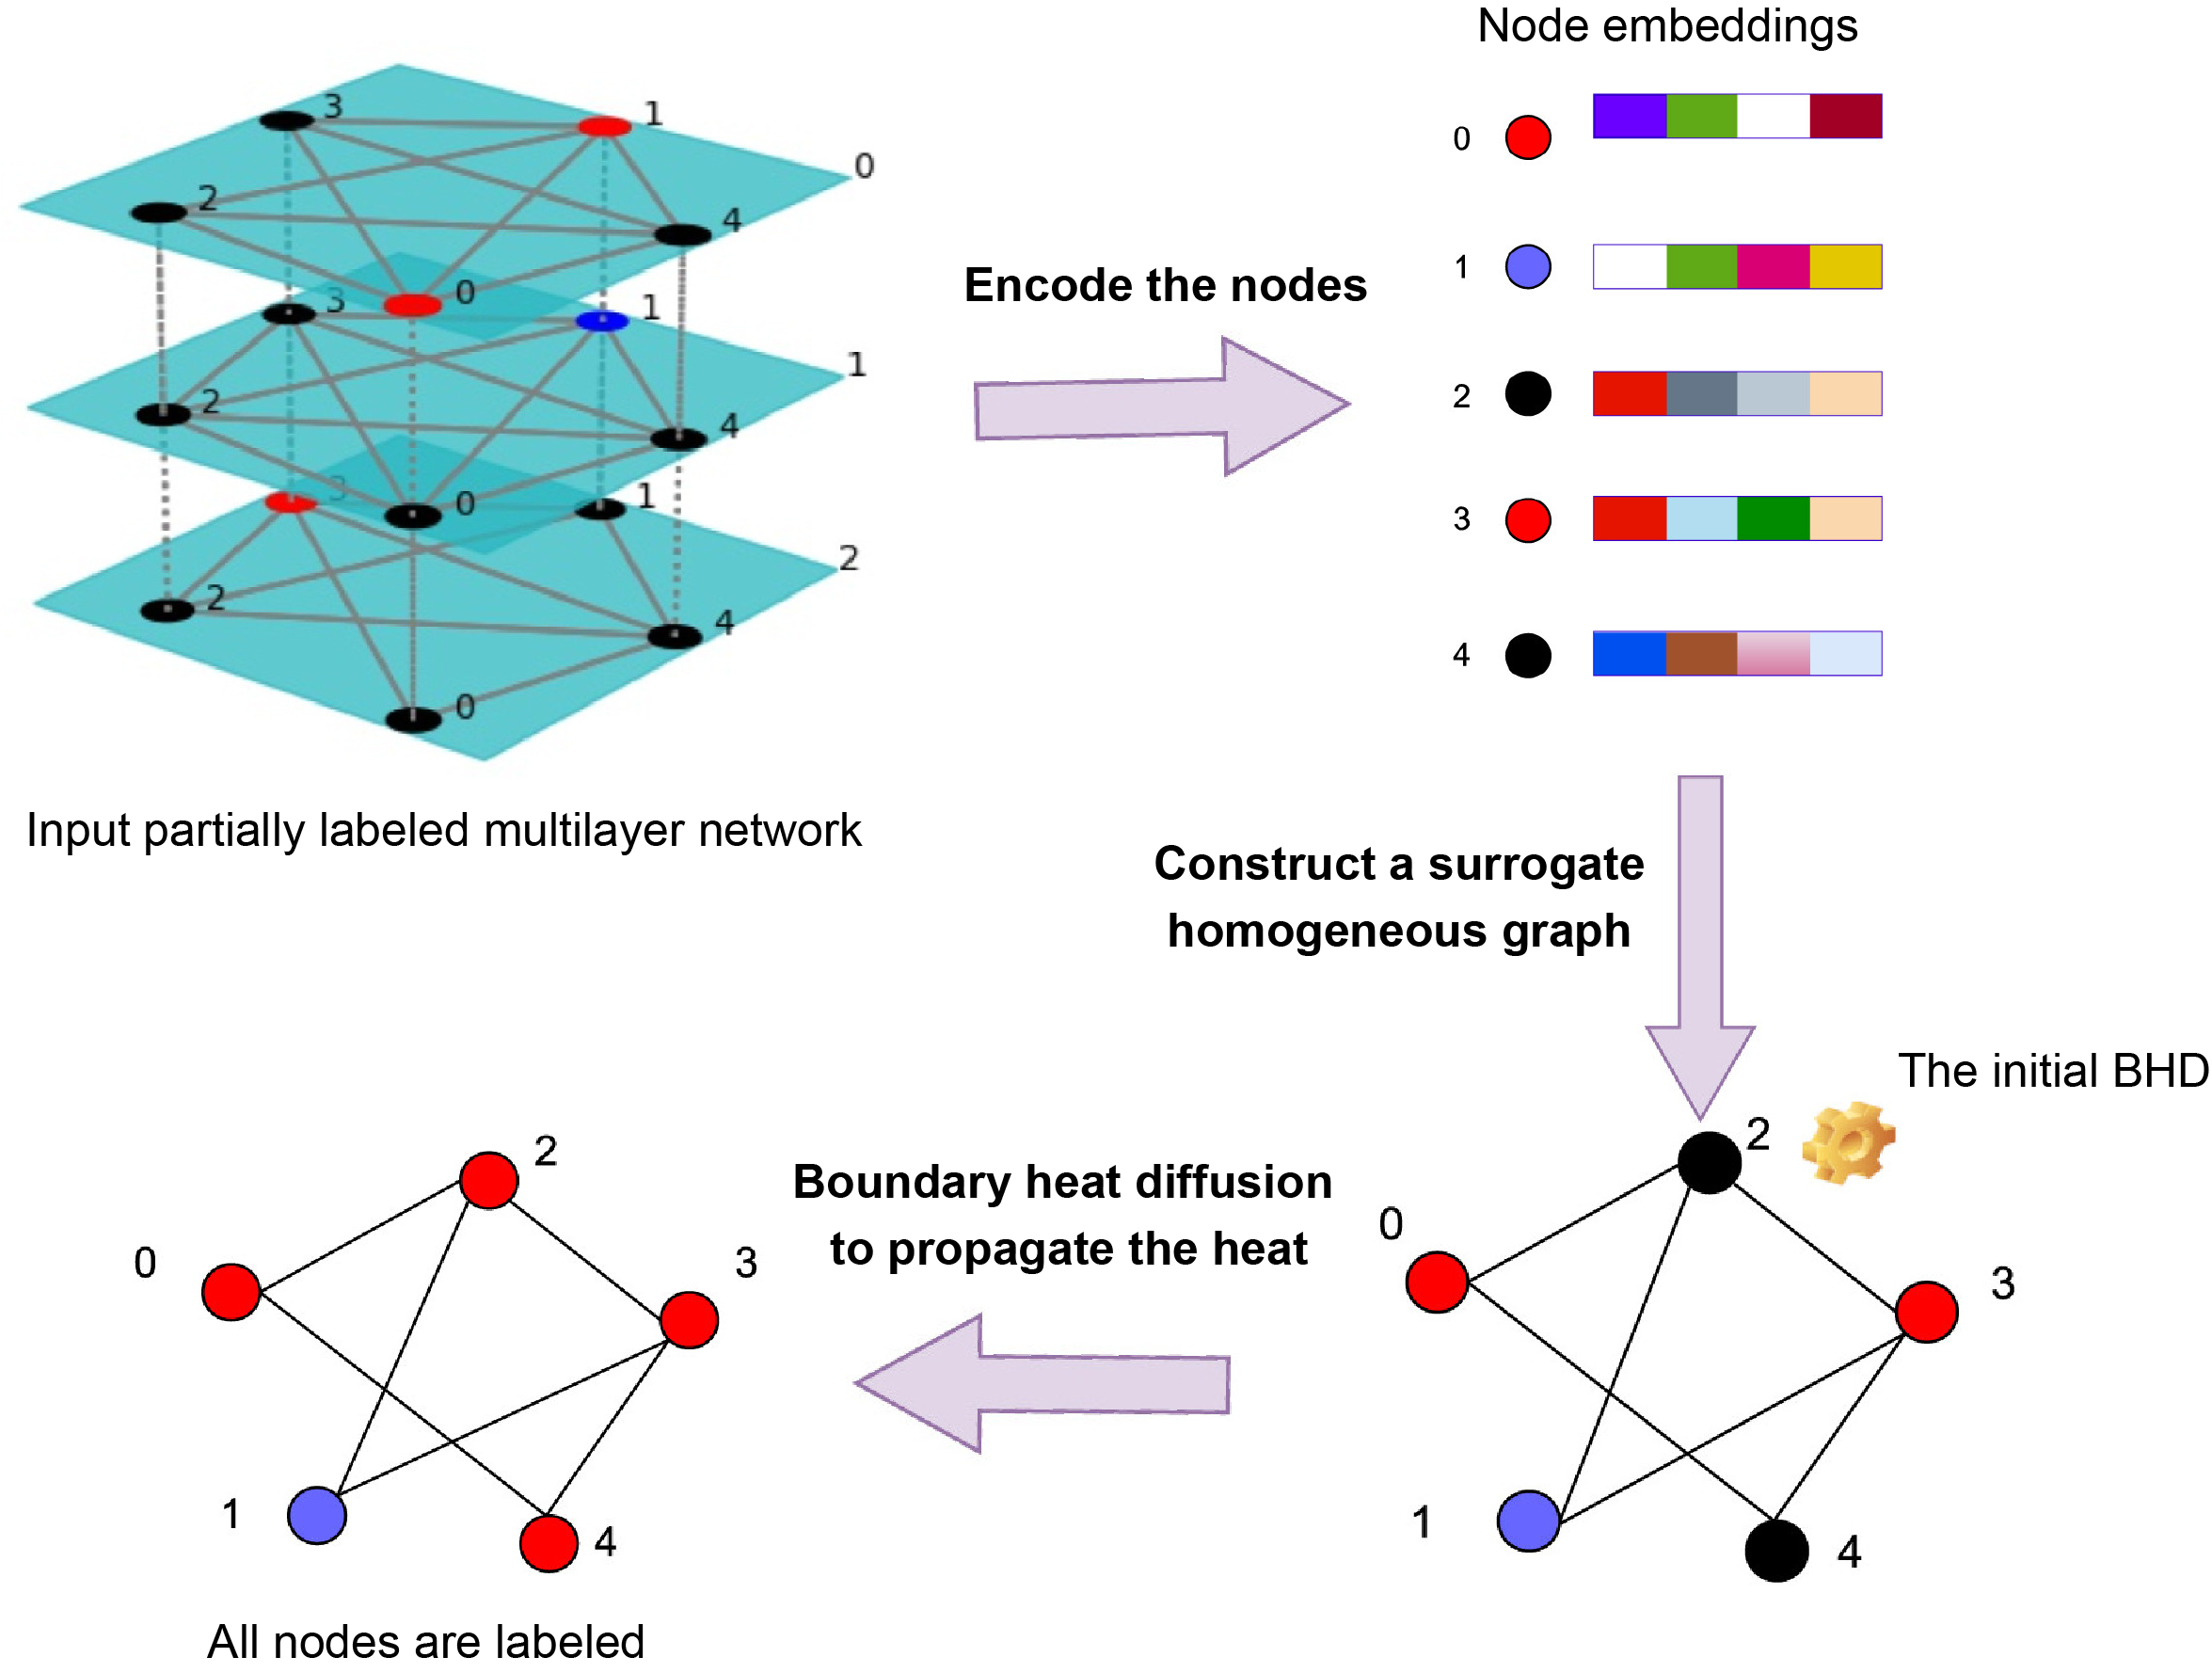
\includegraphics[width=1\textwidth]{Holicheva-Step-3-fig}      
\end{column}
\end{columns}
\bigskip
\end{frame}
\end{document}